% ============================================================
% Articulo 4 — Simulacion del sistema de bioconversion
% Contenido completo (sustituye al esqueleto con TODOs)
% ============================================================

\begin{abstract}
Presentamos la simulacion integral del sistema de bioconversion de residuos
con \emph{Hermetia illucens} instrumentado para la medicion de CO$_2$ y CH$_4$:
un gemelo digital de dimension cero que integra la dinamica larval, el lecho
y el aire interno del contenedor, y una verificacion por dinamica de fluidos
computacional (CFD, FEniCSx/dolfinx) del supuesto de mezcla homogenea en la
camara de cria. Se reportan los escenarios de simulacion E2--E5 del protocolo
experimental y las metricas de mezcla que condicionan la instrumentacion.
En el regimen laminar analizado, ninguna configuracion de puertos de
ventilacion logra homogeneizar la camara en la fase ventilada ($\tau_{mix} >
720$ s frente a $\tau_{aire} \approx 175$ s); en cambio, un ventilador pequeno
en la tapa homogeneiza la camara sellada en menos de 60 s, validando la fase
de cierre estatico del protocolo de medicion.

\textbf{Palabras clave:} bioconversion, \emph{Hermetia illucens}, gemelo
digital, CO$_2$, CH$_4$, dolfinx.
\end{abstract}

\section{Introduccion}
La bioconversion de residuos organicos con larvas de \emph{Hermetia illucens}
(mosca soldado negra) es una alternativa emergente al compostaje y al
relleno sanitario, con produccion simultanea de proteina y abono
\parencite{goldBiowasteTreatmentBlack2020,surendraBioconversionOrganicWastes2016}.
La intensificacion del proceso exige cuantificar sus emisiones de gases de
efecto invernadero (GEI): CO$_2$ de origen biogenico y, en condiciones
anoxicas parciales, CH$_4$ \parencite{boakye-yiadomGreenhouseGasEmissions2022,
ermolaevGreenhouseGasEmissions2019,parodiBioconversionEfficienciesGreenhouse2020a}.
En sistemas de cria intensiva instrumentados, la medicion se realiza con
sensores de bajo costo \parencite{dubeyLowCostCO2NDIR2024,
kiplimoAddressingLowCostMethane2024,mitchellCalibrationLowCostMethane2024}
dentro de una camara de cria donde la ventilacion conmuta entre fase abierta
(renovacion de aire controlada) y cierres estaticos para estimar tasas de
emision a partir de la acumulacion de concentracion
\parencite{bertinMeasuringMethaneEmissions2026}.

El supuesto que hace validas estas mediciones es que el aire interno esta
bien mezclado (supuesto A1): si la concentracion es espacialmente uniforme,
la tasa de emision se obtiene de la pendiente de concentracion sin necesidad
de conocer el campo de flujo completo. Este articulo valida por simulacion el
diseno de la camara antes de la campana experimental, con dos herramientas
complementarias: (i) un gemelo digital de dimension cero (0D) que integra
la dinamica larval, el lecho de sustrato y el aire interno, con el calendario
de cierres del protocolo; y (ii) un modelo CFD estacionario del aire de la
camara que verifica el supuesto A1 y cuantifica las metricas de mezcla
($\tau_{mix}$, $\tau_{aire}$) para distintas configuraciones de puertos y
para mezcla forzada con un ventilador interno.

\section{Modelo del sistema}
\subsection{Dinamica 0D: doce estados}
El gemelo digital (documento de modelo matematico del repositorio) tiene doce
estados: reserva y estructura larvaria ($A$, $B$), longitud ($L$), poblacion
($N$), sustrato disponible ($S$), humedad y temperatura del lecho
($\theta_s$, $T_s$), y temperatura, humedad absoluta y concentraciones del
aire interno ($T$, $w$, $c_{CO_2}$, $c_{O_2}$, $c_{CH_4}$). La cinética larval
sigue el modelo dinamico de \textcite{eriksenDynamicModellingFeed2022} con
parametros metabolicos de \textcite{eriksenMetabolicPerformanceFeed2024}; el
balance de gases incluye respiracion larvaria, actividad microbiana del lecho
y transferencia con el aire renovado por la ventilacion. El estado se propaga
con \texttt{scipy.solve\_ivp} (metodo BDF, por rigidez del sistema acoplado).

\subsection{Entradas conmutadas y cierres}
Las entradas de aire toman una forma unificada para las fases ventilada y
cerrada: con la ventilacion activa, los gases se renuevan a caudal $Q(t)$
modulado por un controlador PI que mantiene el O$_2$ en banda operativa;
durante un cierre, $Q = 0$ y la concentracion evoluciona por acumulacion pura,
$\mathrm{d}c/\mathrm{d}t = r_{emis}/V_{aire}$, de donde se estima la tasa
$r_{emis}$ por ajuste de pendiente. La duracion del cierre $\Delta$ esta
acotada inferiormente por la resolucion del sensor y superiormente por la
linealidad de la pendiente y la acumulacion de CH$_4$. El calendario es
adaptativo: el $\Delta$ del dia siguiente se ajusta segun la pendiente
observada en el cierre anterior, lo que mantiene la resolucion sin saturar
los sensores.

\section{Simulacion del sistema dinamico}
\subsection{Implementacion}
Python 3 + SciPy; parametros de \textcite{eriksenDynamicModellingFeed2022,
eriksenMetabolicPerformanceFeed2024}. El codigo, las figuras y los
resultados estan versionados en el repositorio del proyecto.

\subsection{Escenarios E2--E5}
Se simularon los escenarios E2--E5 del protocolo experimental; la Figura
\ref{fig:escenarios} muestra los escenarios E2 (densidad inicial
$N_0 = 400$ larvas) y E5 ($N_0 = 700$ larvas): concentraciones de CO$_2$,
O$_2$ y CH$_4$, temperaturas del aire y del lecho, y masa del lote. En ambos
casos el controlador de O$_2$ mantiene la concentracion dentro de la banda
operativa y los cierres capturan pendientes de acumulacion distinguibles
sobre el ruido.

\begin{figure}[htbp]
  \centering
  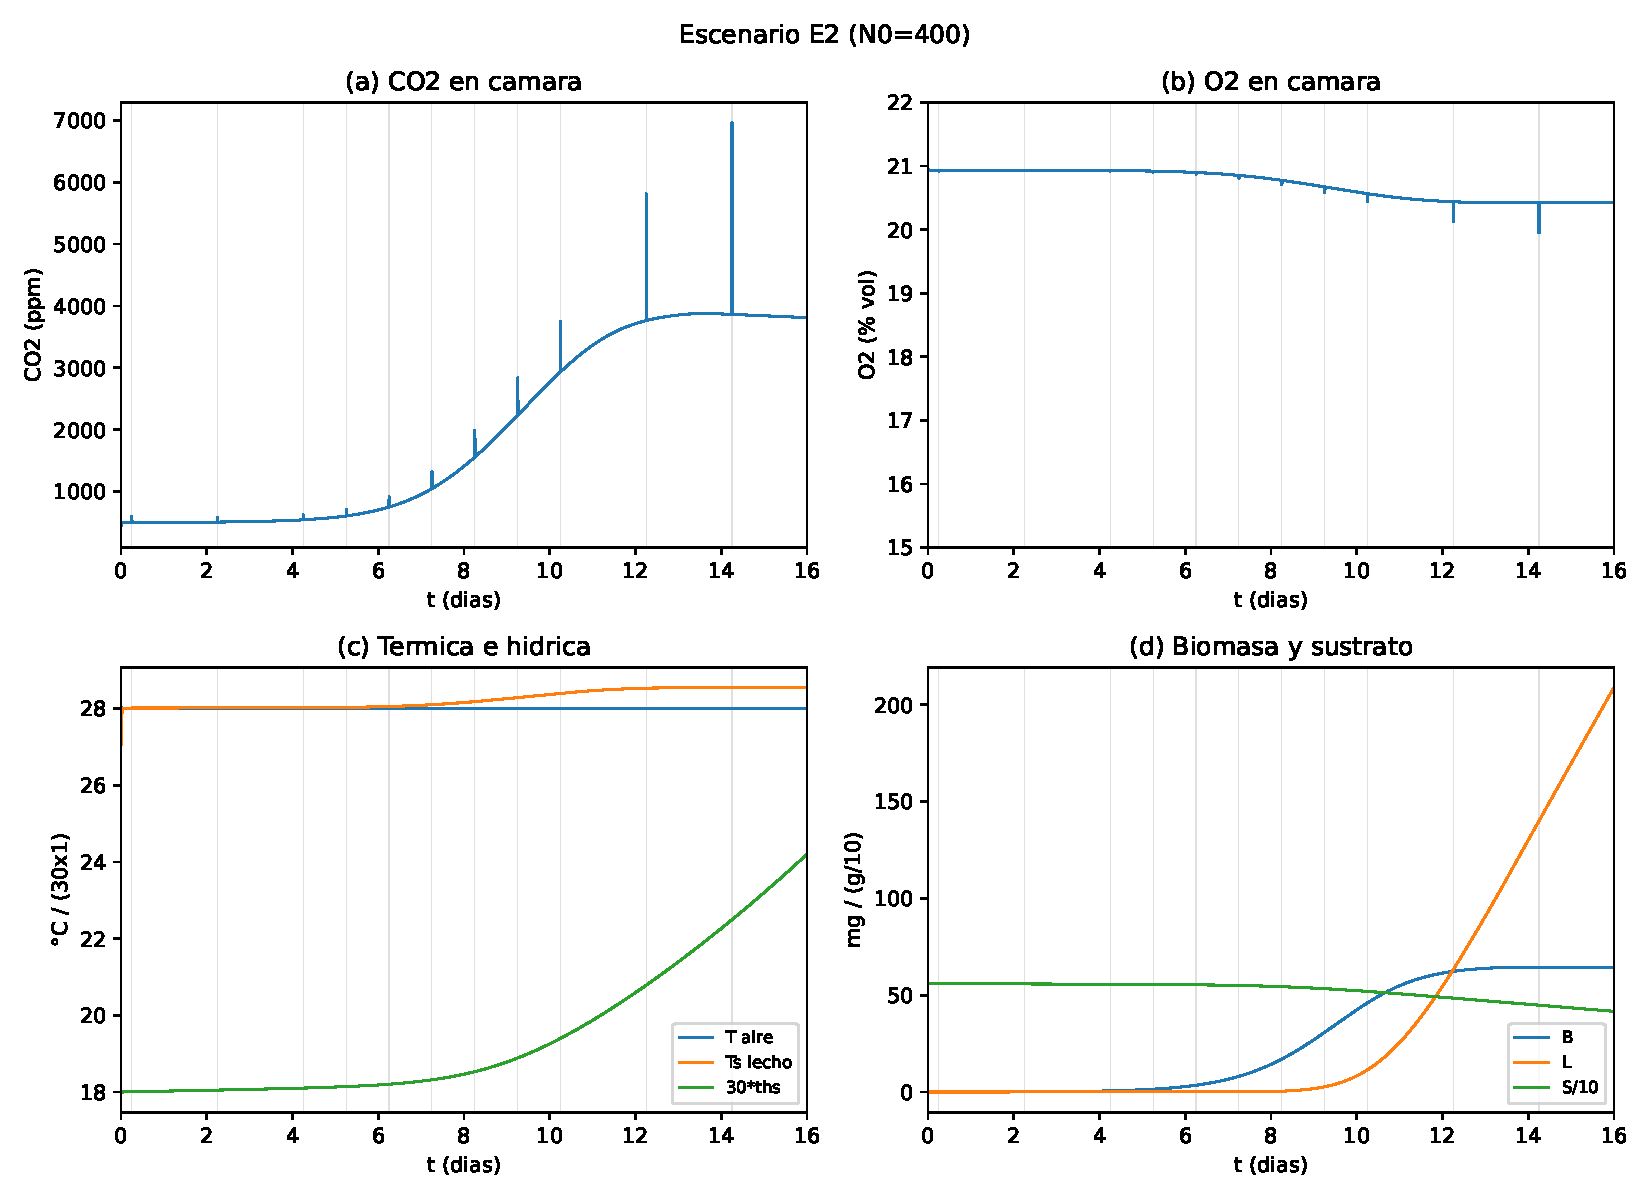
\includegraphics[width=\textwidth]{imagenes/sim_E2.pdf}\\[2mm]
  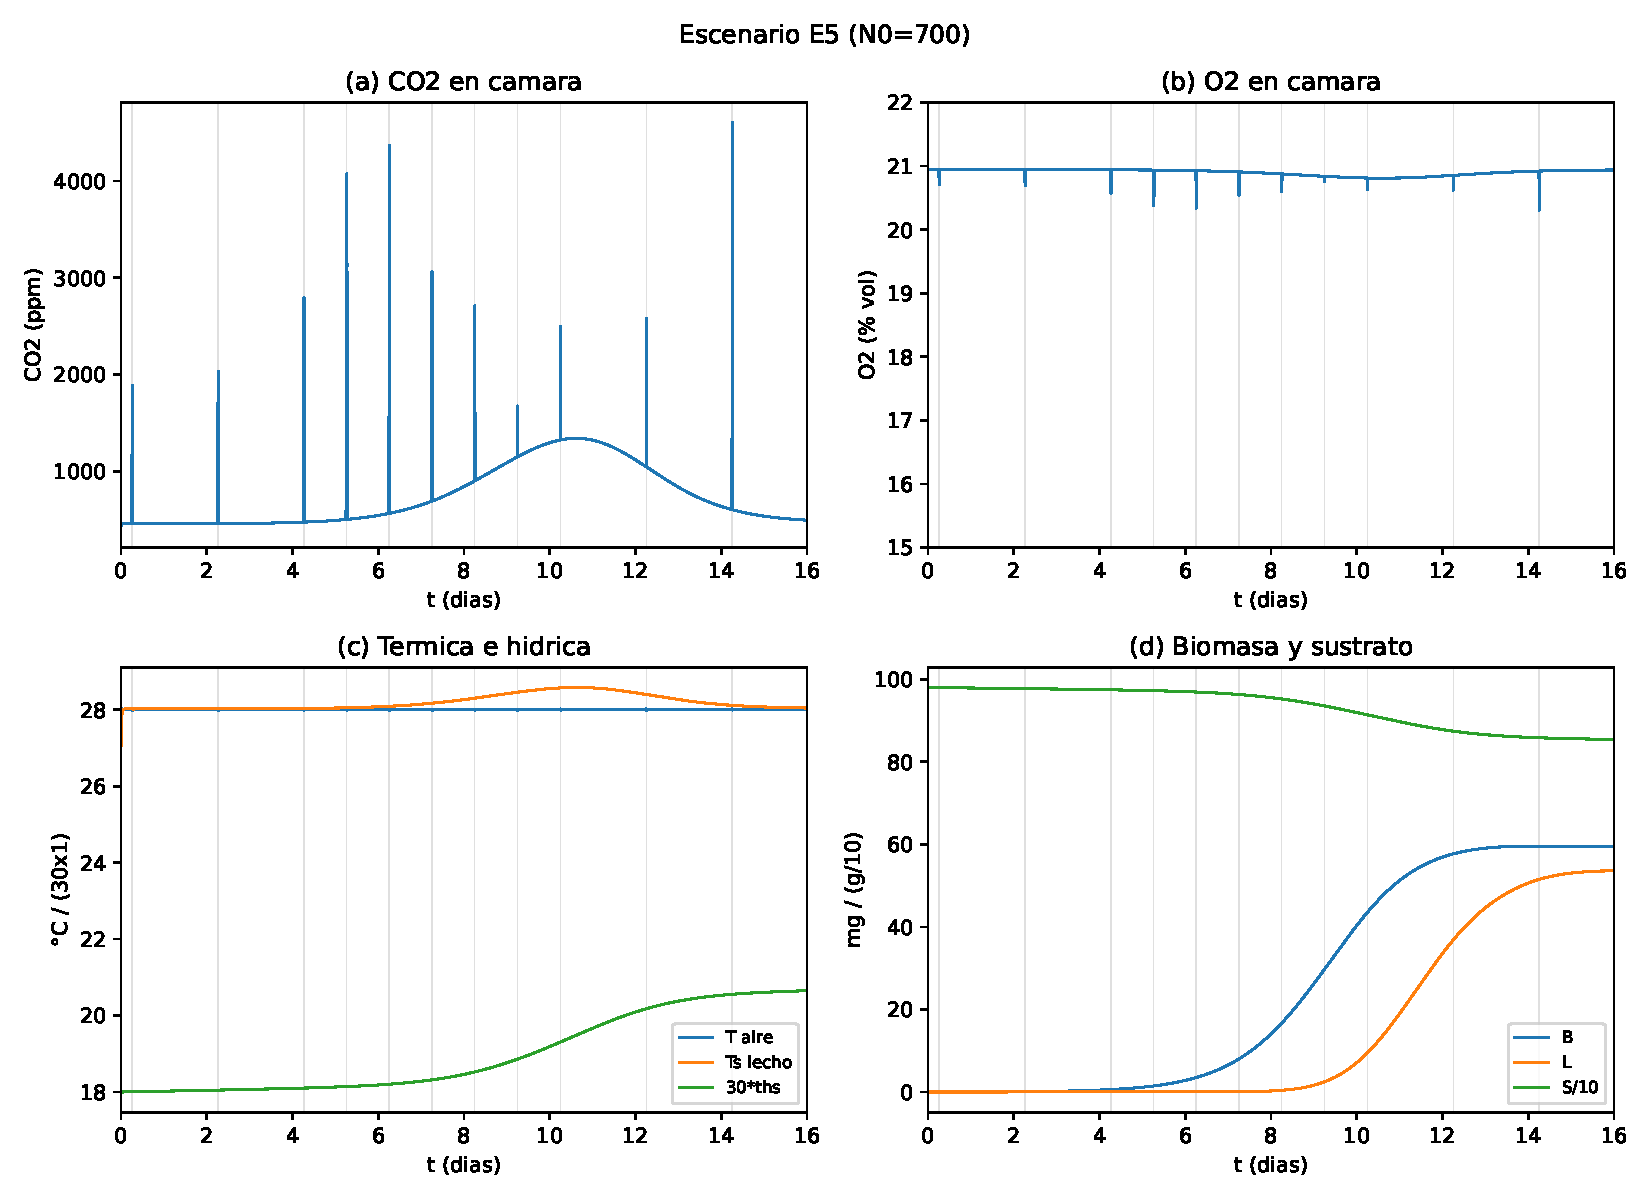
\includegraphics[width=\textwidth]{imagenes/sim_E5.pdf}
  \caption{Escenarios E2 ($N_0 = 400$, arriba) y E5 ($N_0 = 700$, abajo):
  concentraciones de CO$_2$ y O$_2$, variables termicas y masa del lote.
  Las excursiones verticales de CO$_2$ marcan los cierres de medicion.}
  \label{fig:escenarios}
\end{figure}

\subsection{Cierres adaptativos}
La duracion del cierre se adapta dia a dia a la tasa del cierre anterior: con
tasas altas (inicio de la cria) los cierres se acortan para no saturar el
rango de los sensores, y con tasas bajas se alargan para conservar resolucion.
Se evaluo ademas la sensibilidad al volumen de aire efectivo $V_{aire}$:
una incertidumbre de $\pm 20\,\%$ en $V_{aire}$ se traduce directamente en
igual incertidumbre en las tasas estimadas, lo que justifica su calibracion
experimental por dilucion de un trazador.

\section{Verificacion CFD de la mezcla}
\subsection{Geometria y malla}
La camara es un contenedor de $26 \times 19 \times 18$ cm
($\approx 8.9$ L geometricos) empleado para conservar la temperatura del
lote, con un volumen de aire efectivo $V_{aire} = 2.5$ L sobre el lecho de
cria; el trazador se inicializa en la zona del lecho ($c = 1$ en $z < 0.05$ m). La malla se genero con gmsh: discos conformales de puerto
(radio 3 mm) sobresaliendo 1 mm de la cara para garantizar su reconocimiento
en el mallado, fragmentados con el volumen y puntos de refinamiento local
(tamano 1--1.5 mm) que resuelven el chorro de entrada; resultado
$\sim 32\,000$ tetraedros con elementos P2. Las fronteras se marcaron por
centroide geometrico (la lectura aborta si el mallado lleva grupos fisicos
en superficies); los puertos de entrada y salida quedaron con 29 facetas cada
uno, verificando la resolucion local.

\subsection{Modelo de flujo}
Flujo incompresible estacionario en regimen de Stokes penalizado
($\mu = 1.9\times10^{-5}$ Pa·s, $\lambda = 10^4 \mu$), con condiciones de
Dirichlet de caudal en ambos puertos ($Q = 1$ L/min, velocidad de puerto
$U_{in} = 0.589$ m/s, $\mathrm{Re} \approx 220$ en el puerto, transicional) y
paredes sin deslizamiento. El transporte de CO$_2$ se modela como
adveccion-difusion de un escalar pasivo ($D_{CO_2} = 2\times10^{-5}$ m$^2$/s)
con estabilizacion SUPG e integracion implicita de Euler con $\Delta t = 2$ s;
el trazador se inicializa en el lecho ($c = 1$ en $z < 0.05$ m) y la entrada
impone $c = 0$. Las condiciones de contorno se aplicaron por subespacios
vectoriales con verificacion post-solucion (en dolfinx 0.11 un \texttt{Constant}
vectorial sobre el espacio bloqueado falla silenciosamente). El regimen de
Stokes es una cota conservadora: al ignorar la inercia y la turbulencia del
chorro real (Re $\approx 220$), el modelo subestima sistematicamente la mezcla.

\subsection{Metricas de mezcla}
Se define el indice de heterogeneidad $\eta(t) = \sigma_c(t)/\bar{c}_0$ y el
tiempo de mezcla $\tau_{mix}$ como el primer instante con $\eta < 0.05$. En
fase ventilada comparamos contra $\tau_{aire} = V_{aire}/Q_{eff}$, con
$Q_{eff} = (|q_{in}| + q_{out})/2$ medido sobre las fronteras (el caudal
efectivo resulta 15--18\% inferior al nominal por el efecto de banda del
borde del puerto). El fraccionamiento de la camara se evalua comparando la
masa de trazador remanente contra el decaimiento del reactor ideal
$e^{-t/\tau_{aire}}$.

\subsection{Escenarios de puertos en fase ventilada}
Se barrio la posicion de los puertos: C1v2 (entrada lateral baja, salida
lateral alta), C2v2 (entrada en tapa, chorro vertical) y C4v2 (entrada
inclinada 45$^\circ$). Una configuracion con entrada tangencial (C3) se
descarto porque inyecta masa nula en Stokes (artefacto de succion). La
Figura~\ref{fig:tau_mix} (izquierda) muestra que en ningun caso $\eta$ cruza
el umbral: $\tau_{mix} > 720$ s en las tres configuraciones, con
$\eta(720\,\mathrm{s}) = 0.246/0.114/0.110$ y masa remanente
$36.5/17.2/18.5\,\%$ para C1v2/C2v2/C4v2 (Tabla~\ref{tab:cfd}), es decir
$\tau_{mix}/\tau_{aire} > 4$: sin inercia, la geometria de puertos por si
sola no sostiene el supuesto A1 en fase ventilada.

\begin{table}[htbp]
  \centering
  \caption{Resultados CFD. Fase ventilada: $Q = 1$ L/min en ambos puertos.
  Fase cerrada: camara sellada con ventilador (fuente de momentum).}
  \label{tab:cfd}
  \begin{tabular}{lcccc}
    \hline
    Config. & $Q_{eff}$ (L/min) & $\tau_{aire}$ (s) & $\eta(720\,\mathrm{s})$ &
    $\tau_{mix}$ (s) \\
    \hline
    C1v2 & 0.857 & 175 & 0.246 & $> 720$ \\
    C2v2 & 0.899 & 167 & 0.114 & $> 720$ \\
    C4v2 & 0.845 & 177 & 0.110 & $> 720$ \\
    C5cerrada ($F_0 = 400$) & 0 (sellada) & $\infty$ & --- & 4 \\
    C5cerrada\_F4 ($F_0 = 4$) & 0 (sellada) & $\infty$ & --- & 24 \\
    \hline
  \end{tabular}
\end{table}

\subsection{Mezcla forzada con ventilador en tapa (C5)}
Se modelo un ventilador axial pequeno (40 mm) en la tapa, directamente sobre
las larvas, como una fuente de momentum (fuerza corporal $-\mathbf{z}$)
dentro de una esfera de radio 2 cm bajo la tapa; este modelo inyecta el
momento del ventilador sin mallar las aspas. El escenario de interes es la
camara sellada ($Q = 0$ en ambos puertos), que reproduce exactamente la fase
de cierre del protocolo. La Figura~\ref{fig:tau_mix} (derecha) muestra el
decaimiento de $\eta$: $\tau_{mix} = 4$ s con $F_0 = 400$ N/m$^3$ y
$\tau_{mix} = 24$ s con $F_0 = 4$ N/m$^3$ (velocidad maxima 1101.8 y
11.02 m/s respectivamente). El escalamiento lineal de Stokes se verifico de
forma exacta (100$\times$ menos fuerza = 100$\times$ menos velocidad), y la
mezcla satura: para cualquier fuerza significativa la camara se homogeniza
en menos de 60 s, con deriva de masa inferior al 1\% en sellado perfecto.
Como el regimen real del ventilador es transicional-turbulento, estos tiempos
son una cota conservadora de la mezcla real.

\begin{figure}[htbp]
  \centering
  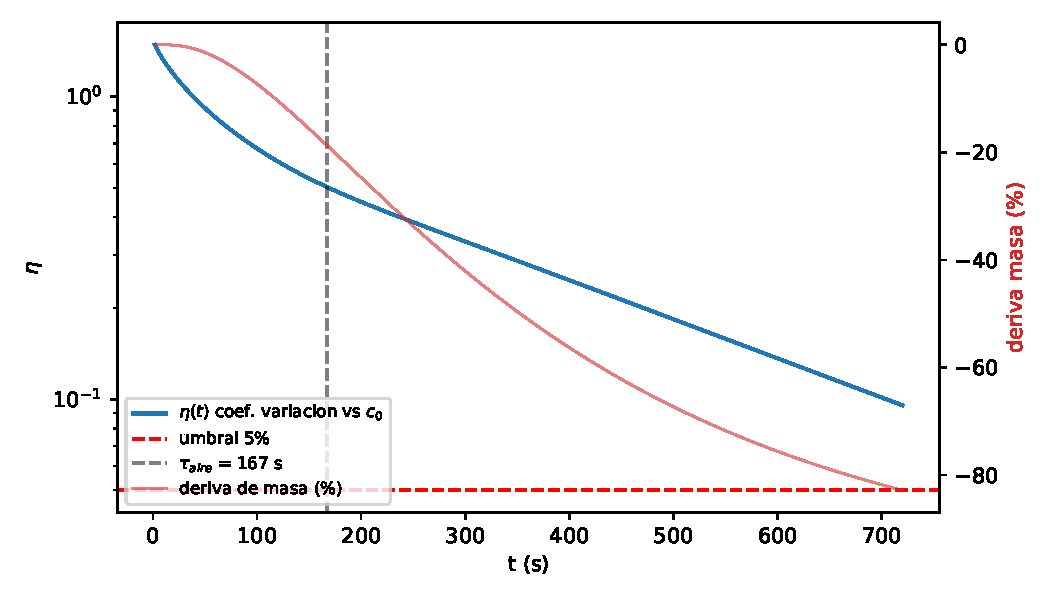
\includegraphics[width=0.48\textwidth]{imagenes/cfd_tau_mix_C2v2.pdf}\hfill
  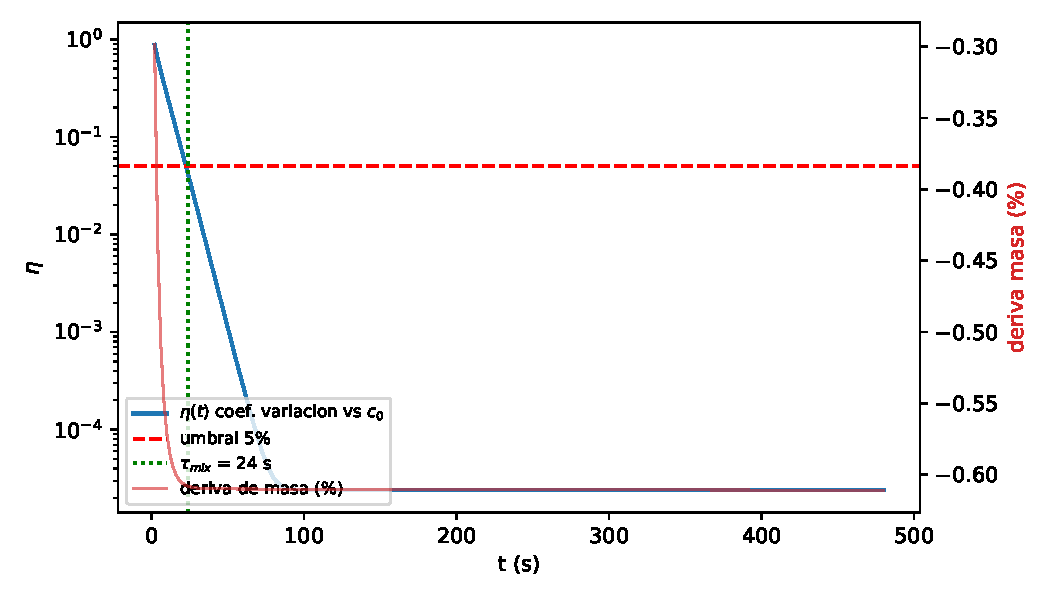
\includegraphics[width=0.48\textwidth]{imagenes/cfd_tau_mix_C5cerrada_F4.pdf}
  \caption{Izquierda: fase ventilada (C2v2) --- $\eta$ nunca cruza el umbral
  0.05. Derecha: camara sellada con ventilador (C5cerrada\_F4) ---
  $\tau_{mix} = 24$ s.}
  \label{fig:tau_mix}
\end{figure}

\begin{figure}[htbp]
  \centering
  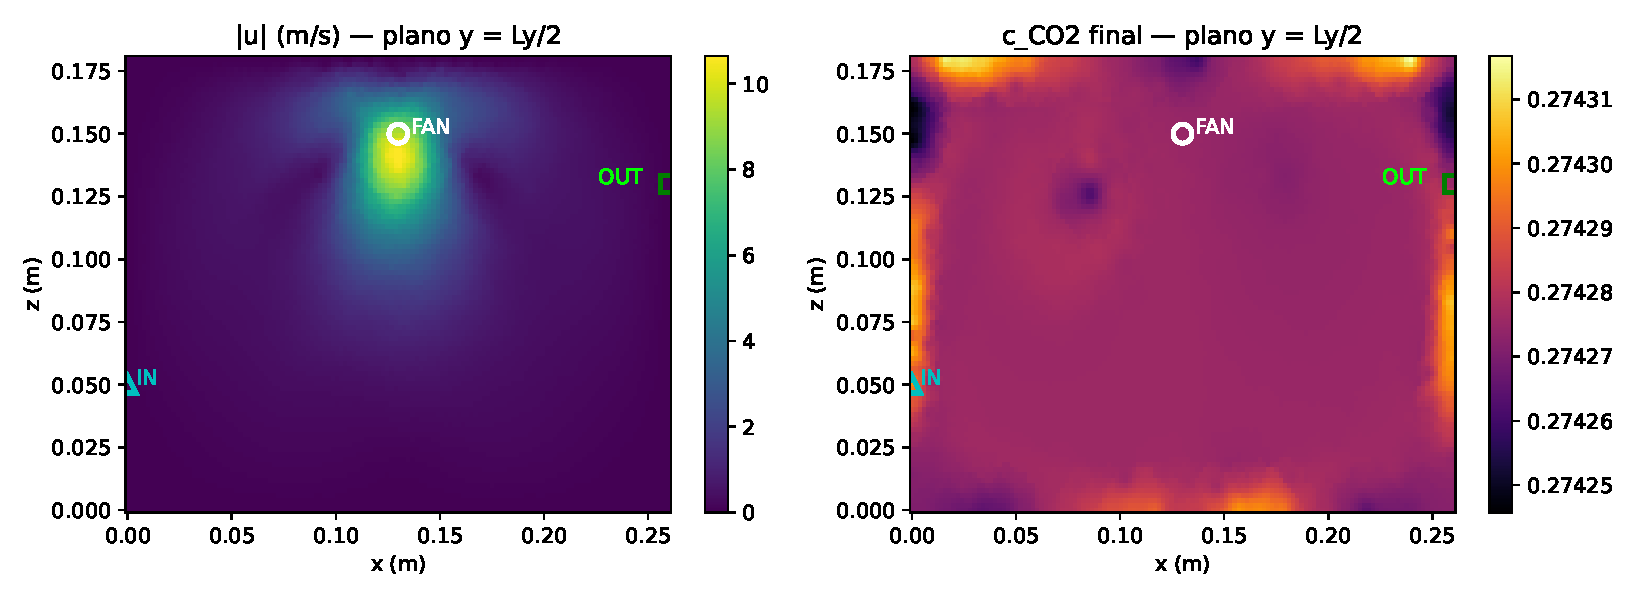
\includegraphics[width=0.7\textwidth]{imagenes/cfd_distribucion_C5cerrada_F4.pdf}
  \caption{Campo de concentracion (interpolacion IDW sobre cortes) de la
  camara sellada con ventilador: el trazador inicialmente concentrado en el
  lecho se homogeneiza en decenas de segundos.}
  \label{fig:campo_c5}
\end{figure}

\section{Resultados y discusion}
La combinacion de resultados fija las condiciones de validez del protocolo de
medicion. En fase ventilada, el gemelo digital 0D proporciona tasas
instantaneas de emision, pero el CFD muestra que el supuesto A1 no se
sostiene con ventilacion por puertos en el regimen analizado: las lecturas
del sensor promedian una camara con zonas muertas, con sesgo hacia las
concentraciones mas altas del entorno del lecho (en C1v2 el 36.5\% del
trazador permanece en la camara a 720 s). Por ello las tasas de fase
ventilada deben tratarse como estimaciones acotadas, no como mediciones de
precision. En fase cerrada, en cambio, el ventilador en tapa garantiza la
homogeneidad en menos de 60 s frente a cierres de 10--30 min: el supuesto A1
queda validado con un margen de 10--30$\times$, y la pendiente de acumulacion
durante el cierre es una medicion de tasa directa y defendible. El diseno
final que emerge es: (i) ventilador fijo (no controlado en velocidad; la
mezcla saturada hace innecesario el control) de material de baja emision en
la tapa centrado sobre las larvas; (ii) medicion del caudal efectivo de los
puertos y de la presion interna de la camara (deteccion de fugas y
correccion); (iii) cierres estaticos para CH$_4$ y validacion cruzada con la
fase ventilada; y (iv) correccion del volumen muerto del gemelo digital a
partir de la fraccion de mezcla observada. La linealidad de Stokes, verificada
en C5, da ademas una ley de diseno sin nuevas simulaciones: $\tau_{mix}$
escala inversamente con el momentum inyectado.

\section{Conclusiones}
\begin{enumerate}
  \item El gemelo digital 0D integra la dinamica larvaria, el lecho y el
  aire interno, y reproduce los escenarios E2--E5 del protocolo con control
  de O$_2$ por ventilacion y cierres adaptativos de duracion dia a dia.
  \item En fase ventilada, ninguna configuracion de puertos homogeneiza la
  camara en regimen laminar: $\tau_{mix} > 720$ s y $\eta(720\,\mathrm{s})
  \geq 0.11$ frente a $\tau_{aire} \approx 175$ s. El supuesto A1 no es
  sostenible en fase abierta sin mezcla forzada.
  \item Un ventilador pequeno en la tapa homogeneiza la camara sellada en
  menos de 60 s ($\tau_{mix} = 4$--$24$ s para un rango de 100$\times$ en la
  fuerza inyectada), validando el supuesto A1 para los cierres de medicion
  con margen de 10--30$\times$.
  \item El escalamiento lineal de Stokes se verifico de forma exacta, lo que
  permite dimensionar el ventilador sin corridas adicionales.
  \item Al ser cotas conservadoras (laminar, isotermo, difusividad
  molecular), los resultados subestiman la mezcla real; la discrepancia se
  cerrara con la calibracion experimental con dos sensores a distinta altura
  y con la correccion de volumen muerto del gemelo digital.
\end{enumerate}

% Figuras usadas:
% fig:escenarios -> sim_E2.pdf, sim_E5.pdf
% fig:tau_mix    -> cfd_tau_mix_C2v2.pdf, cfd_tau_mix_C5cerrada_F4.pdf
% fig:campo_c5   -> cfd_distribucion_C5cerrada_F4.pdf
